% \section{Evolvability \& Genotype-Phenotype Map}

\begin{frame}{Defining Evolvability}
consensus: the amount of \textcolor{h2}{viable} \textcolor{h1}{variation} generated by the evolutionary process
\begin{itemize}
  \item evolvability as the amount of \textcolor{h1}{\textbf{novel variation}} generated
  \item evolvability the proportion of variation that is \textcolor{h2}{\textbf{viable}}
\end{itemize}
\end{frame}

\begin{frame}{Evolvability: Novelty}


\begin{figure}
 \centering
    \begin{subfigure}[b]{0.5\textwidth}
        \centering
    	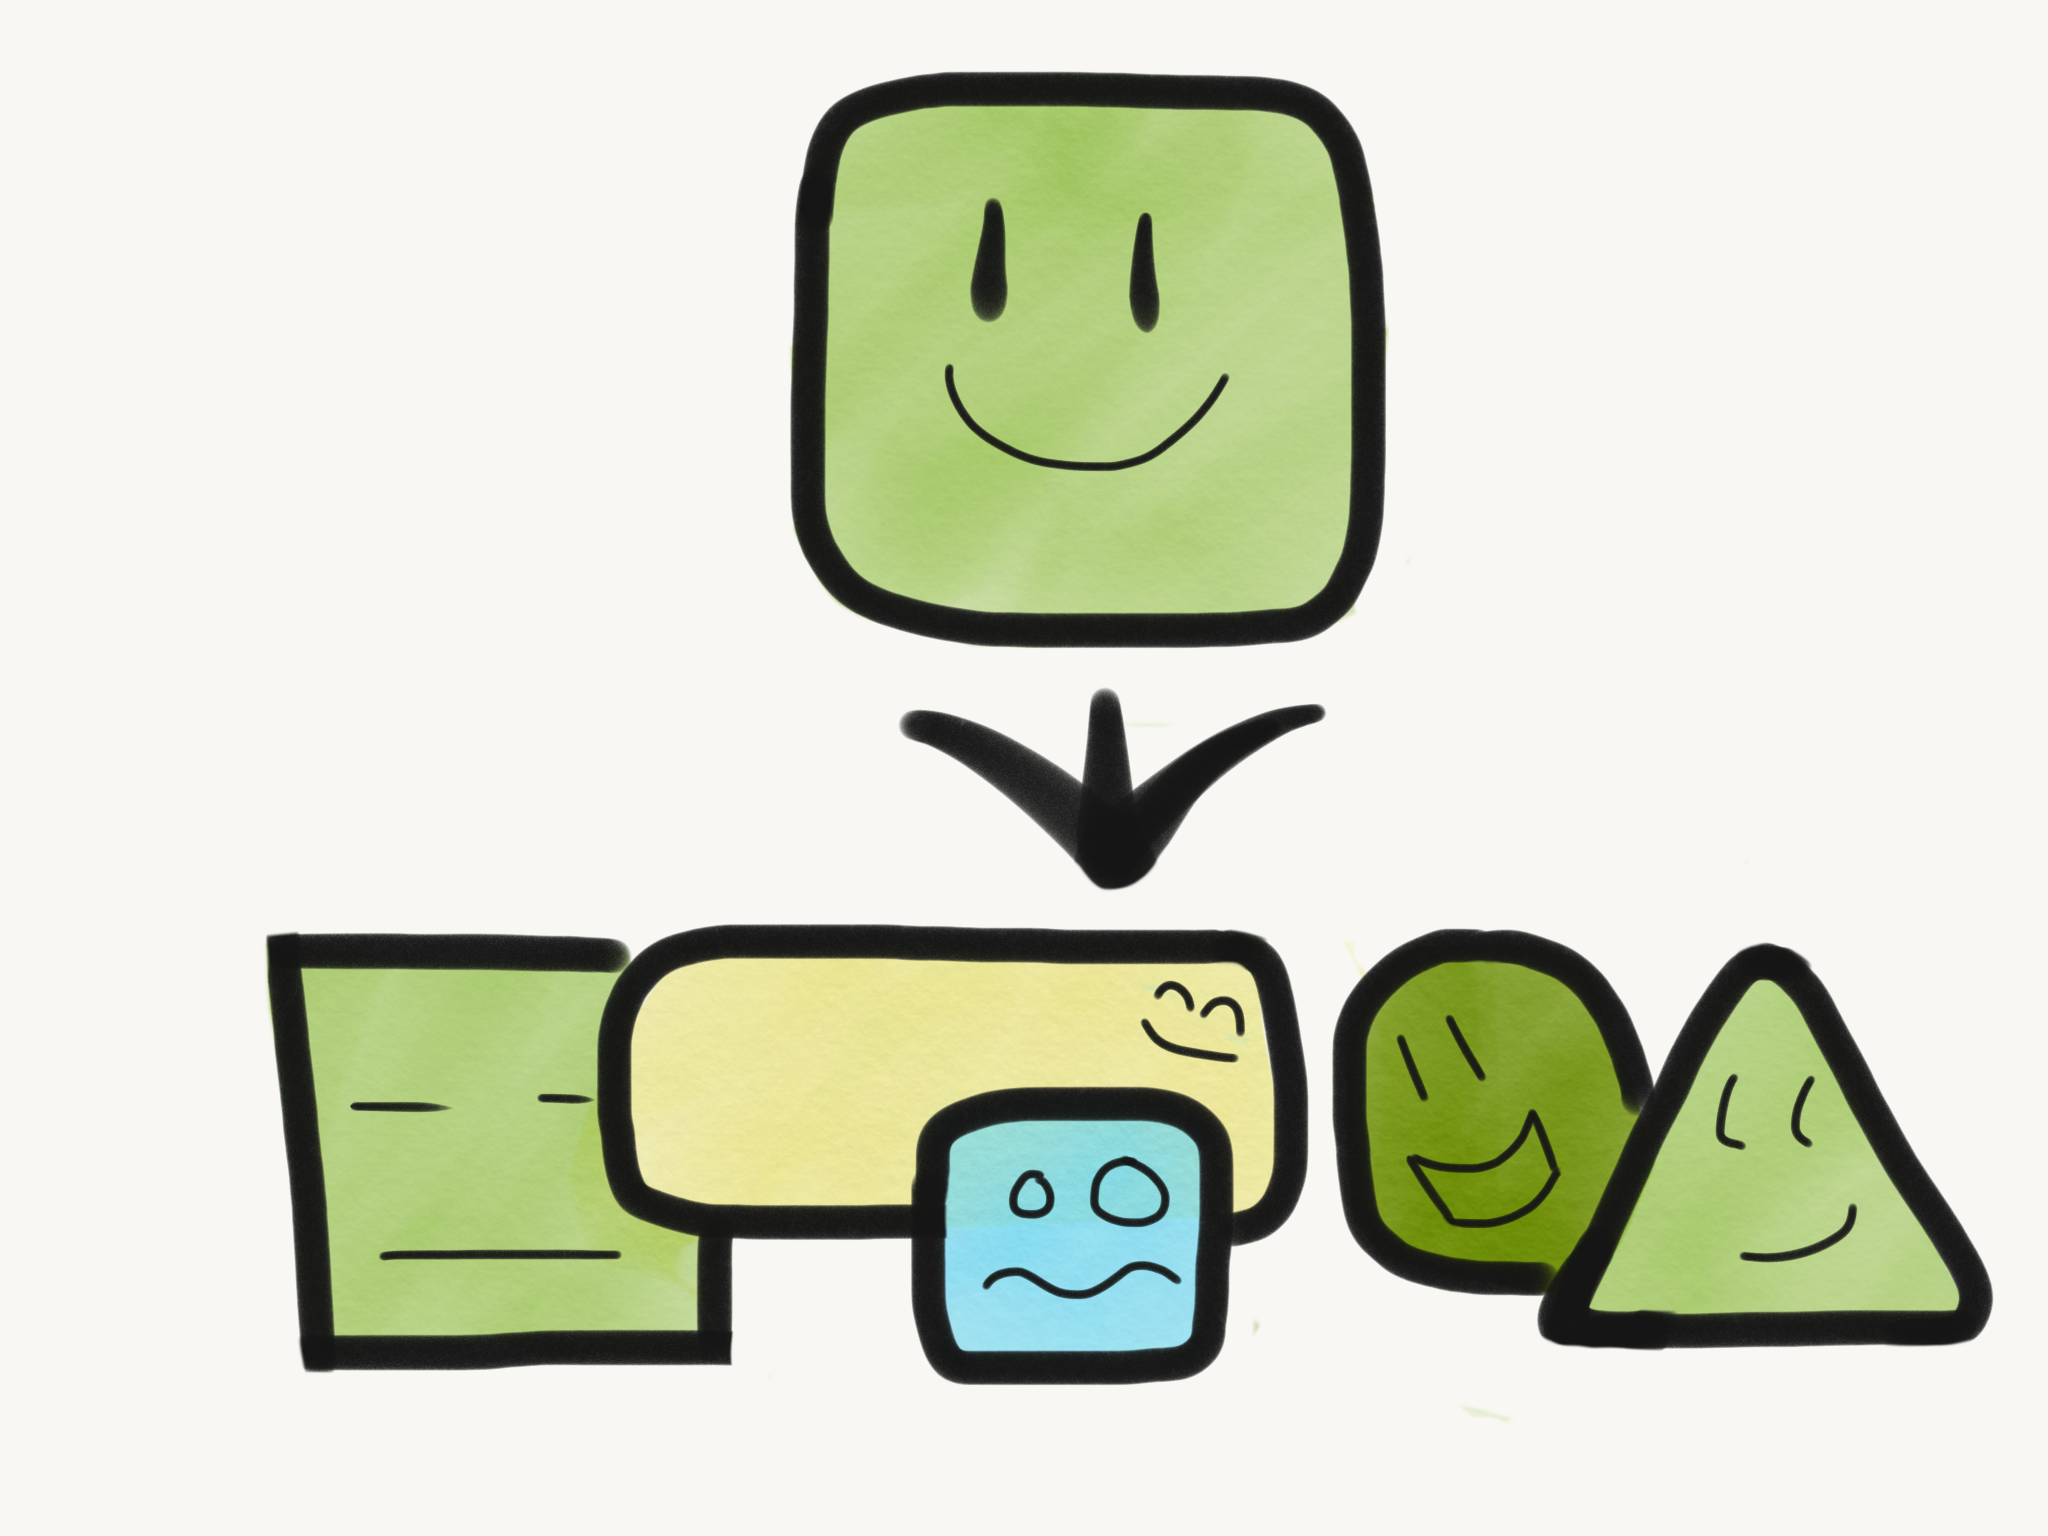
\includegraphics[width=\textwidth]{img/individual_evolvability}
        \caption{high phenotypic variation among offspring}
        \label{fig:high}
    \end{subfigure}%
    \hfill
    \begin{subfigure}[b]{0.5\textwidth}
        \centering
        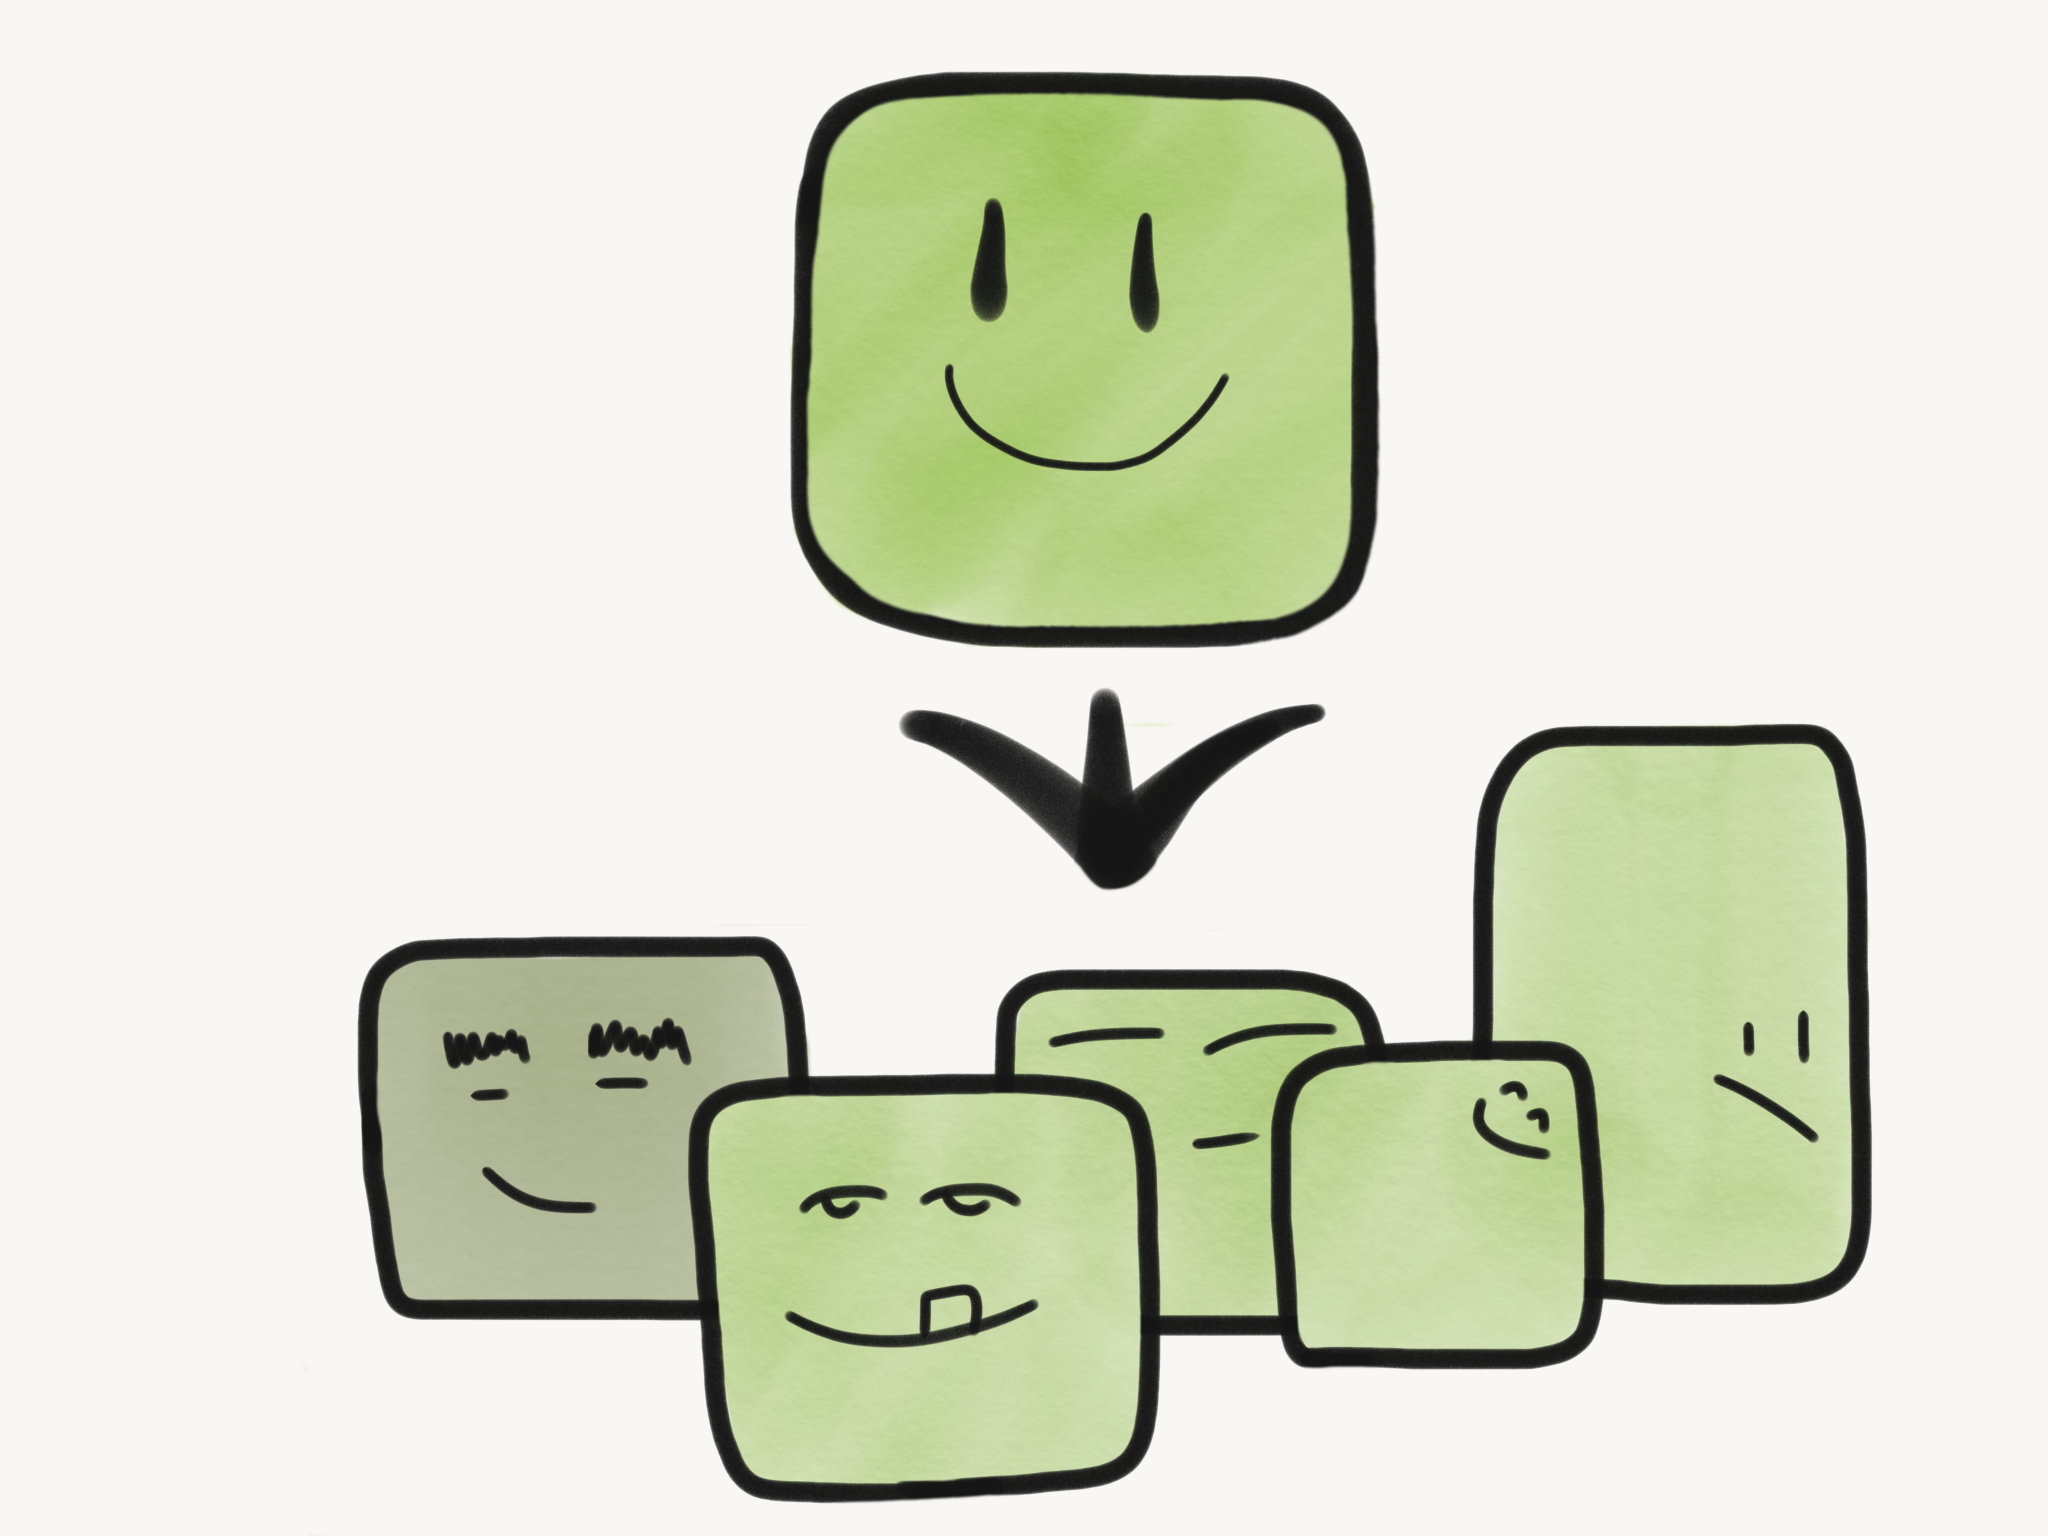
\includegraphics[width=\textwidth]{img/low_individual_evolvability}
        \caption{low phenotypic variation among offspring}
        \label{fig:low}
    \end{subfigure}
    \vspace{-4ex}
  \caption{An comparison of high (\ref{fig:high}) and low (\ref{fig:low}) levels of phenotypic variation under mutation; high evolvability left and low evolvability right.}
\end{figure}


\end{frame}

\begin{frame}{Evolvability: Viability}

\begin{figure}
    \centering
    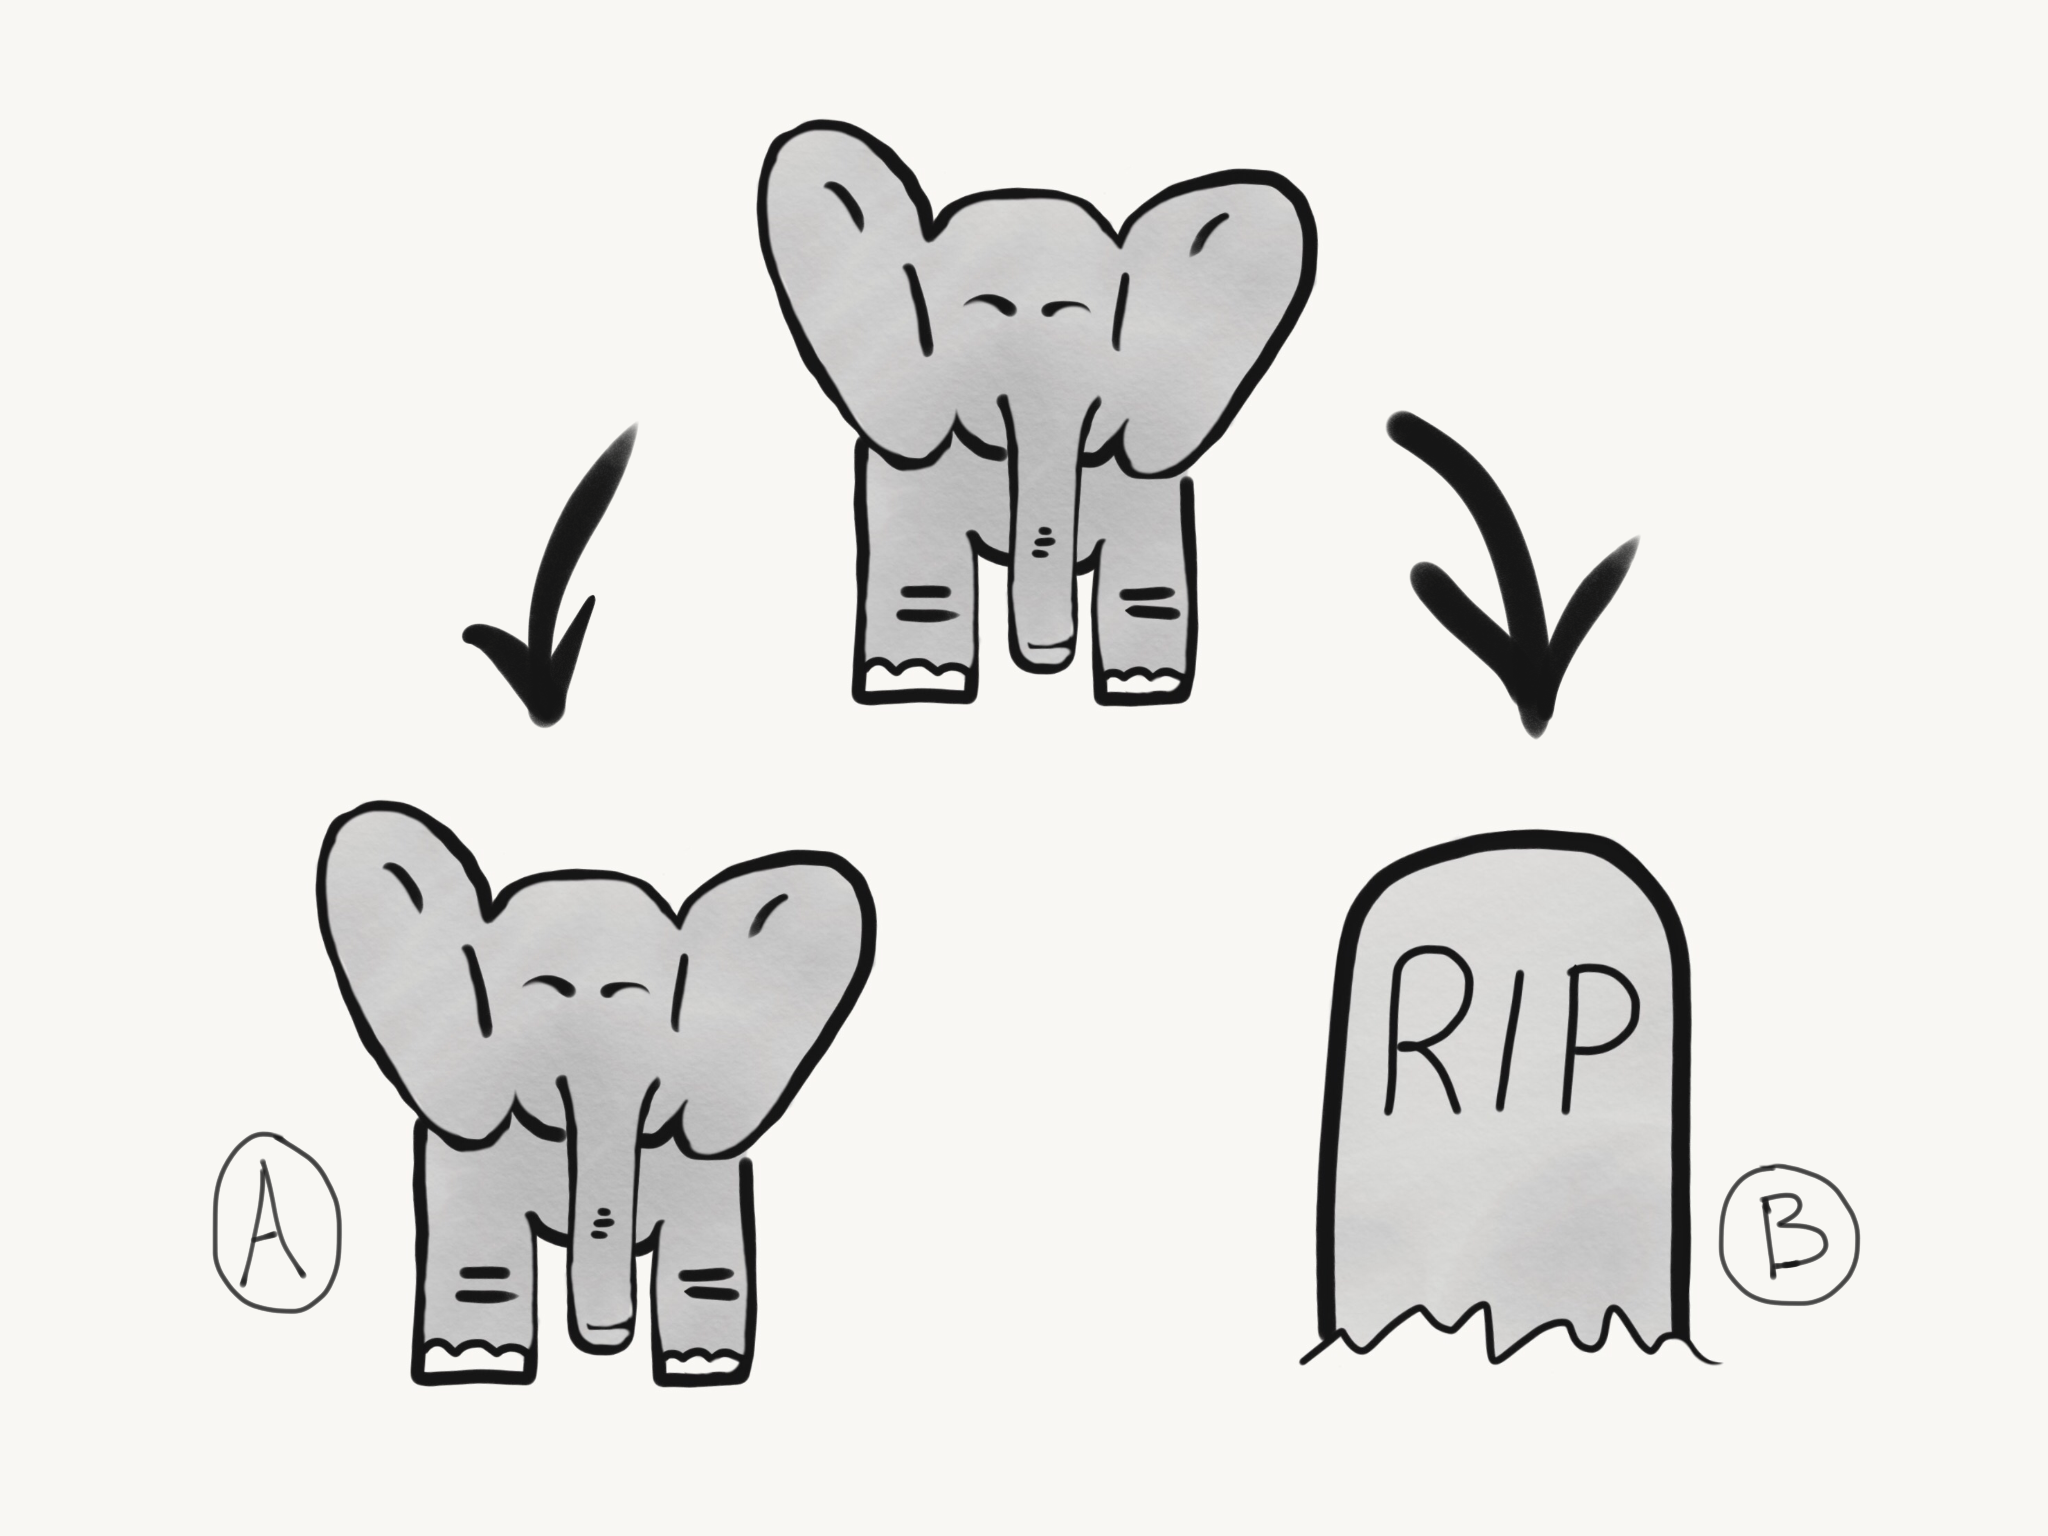
\includegraphics[width=0.8\textwidth]{img/robustness}
 	\captionsetup{singlelinecheck=off,justification=raggedright}
  	\caption{Illustration of robustness under mutation; high evolvability left and low evolvability right.}
    \label{fig:robustness}
\end{figure}


\end{frame}

\begin{frame}{Evolvability \& Genotype-Phenotype Map}

\begin{figure}

\foreach \n in {1,...,4}{%
\includegraphics<\n>[width=0.8\textwidth]{gpmaps/even-\n}%
}%

\caption{
Graph of phenotypes connected by single-step mutations induced by a genotype-phenotype map.
Graphic inspired by \cite{ahnert2017structural}.
}

\end{figure}

\end{frame}

\begin{frame}{Evolvability \& Genotype-Phenotype Map}

\begin{figure}

\foreach \n in {1,...,4}{%
\includegraphics<\n>[width=0.8\textwidth]{gpmaps/filtered-\n}%
}%

\caption{
Graph of phenotypes connected by single-step mutations induced by a genotype-phenotype map.
Note the bias towards viability induced by exclusion of invalid phenotypes.
Graphic inspired by \cite{ahnert2017structural}.
}

\end{figure}

\end{frame}

\begin{frame}{Evolvability \& Genotype-Phenotype Map}

\begin{figure}

\foreach \n in {1,...,4}{%
\includegraphics<\n>[width=0.8\textwidth]{gpmaps/layered-\n}%
}%

\caption{
Graph of phenotypes connected by single-step mutations induced by a genotype-phenotype map.
Note the difficulty of traversing the region of invalid phenotypes.
Graphic inspired by \cite{ahnert2017structural}.
}

\end{figure}

\end{frame}

% \begin{frame}{Evolvability \& Genotype-Phenotype Map}
%
% \begin{figure}
%
% \foreach \n in {1,...,4}{%
% \includegraphics<\n>[width=0.8\textwidth]{gpmaps/rare-\n}%
% }%
%
% \caption{TODO Graphic inspired by \cite{ahnert2017structural}.}
%
% \end{figure}
%
% \end{frame}

\begin{frame}{Evolvability \& Genotype-Phenotype Map}

\begin{figure}

\foreach \n in {1,...,4}{%
\includegraphics<\n>[width=0.8\textwidth]{gpmaps/reduced-\n}%
}%

\caption{
Graph of phenotypes connected by single-step mutations induced by a genotype-phenotype map.
Note the dimensionality reduction.
Graphic inspired by \cite{ahnert2017structural}.
}

\end{figure}

\end{frame}

\begin{frame}{Evolvable Genotype-Phenotype Maps}

\Large

\textcolor{h2}{
In EC, we define the genotype-phenotype map.
}
\normalsize

\vspace{1ex}

\pause

\textbf{Option A:} use direct genotype-phenotype map
\pause
\begin{itemize}
\item often poor evolvability
\end{itemize}

\pause

\textbf{Option B:} use manually-designed indirect genotype-phenotype map
\pause
\begin{itemize}
\item labor-intensive
\item ad-hoc/heuristic
\item might be computationally prohibitive to evaluate
\item might still have poor evolvability$\dots$
\end{itemize}

\pause

\textbf{Option C?}

\end{frame}
